\documentclass[border=10pt]{standalone}
\usepackage{amsmath,amssymb}
\usepackage{tikz}
\usetikzlibrary{arrows.meta,shapes.geometric,shadows,positioning}
\definecolor{acc}{HTML}{0D9488}
\definecolor{ink}{HTML}{1A1D21}
\definecolor{mut}{HTML}{646A72}
\definecolor{bad}{HTML}{E05A47}
\tikzset{
  >=Latex, font=\small,
  q/.style={diamond, aspect=2.6, draw=ink, line width=1.1pt, fill=white, inner sep=1.5pt, align=center, text width=40mm, drop shadow={opacity=0.15}},
  box/.style={rectangle, rounded corners=6pt, draw=acc!75!black, line width=1.2pt, fill=acc!18, minimum height=9mm, align=center, text width=34mm, drop shadow={opacity=0.2}},
  full/.style={box, draw=bad, fill=bad!15},
  pill/.style={rectangle, rounded corners=12pt, draw=mut, line width=1pt, fill=white, minimum height=8mm, align=center, text width=34mm},
  a/.style={->, line width=1.1pt, draw=ink!80},
  lab/.style={font=\footnotesize\itshape, text=mut},
}
\begin{document}
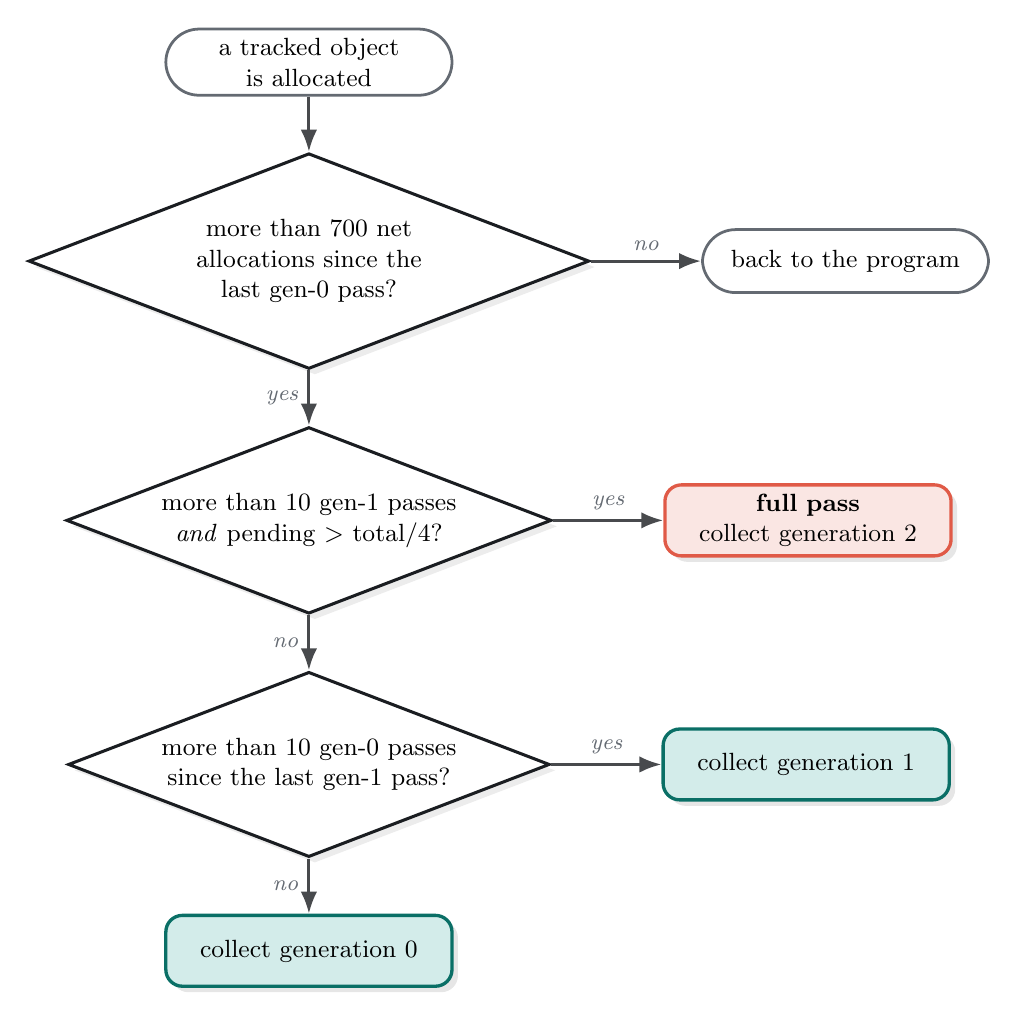
\begin{tikzpicture}[node distance=7mm and 10mm]
  \node[pill] (s) {a tracked object\\is allocated};
  \node[q, below=of s] (q0) {more than 700 net\\allocations since the\\last gen-0 pass?};
  \node[pill, right=14mm of q0] (r) {back to the program};
  \node[q, below=of q0] (q2) {more than 10 gen-1 passes\\\emph{and} pending $>$ total$/4$?};
  \node[full, right=14mm of q2] (f) {\textbf{full pass}\\collect generation 2};
  \node[q, below=of q2] (q1) {more than 10 gen-0 passes\\since the last gen-1 pass?};
  \node[box, right=14mm of q1] (c1) {collect generation 1};
  \node[box, below=of q1] (c0) {collect generation 0};
  \draw[a] (s) -- (q0);
  \draw[a] (q0) -- node[lab, above] {no} (r);
  \draw[a] (q0) -- node[lab, left] {yes} (q2);
  \draw[a] (q2) -- node[lab, above] {yes} (f);
  \draw[a] (q2) -- node[lab, left] {no} (q1);
  \draw[a] (q1) -- node[lab, above] {yes} (c1);
  \draw[a] (q1) -- node[lab, left] {no} (c0);
\end{tikzpicture}
\end{document}
